\documentclass[a4paper]{article}

\usepackage[ngerman]{babel}
\usepackage[utf8]{inputenc}
\usepackage{amsmath}
\usepackage{amssymb}
\usepackage{amsthm}
\usepackage{booktabs}
\usepackage{array}
\usepackage{tabularx}
\usepackage{color}
\usepackage{ulem}
\usepackage{fancyhdr}
\usepackage{graphicx}
\usepackage{geometry}
\usepackage{polynom}
\usepackage{pgf,tikz}
\usepackage{amsfonts}
\usepackage{cancel}
\usepackage{mathcomp}
\usepackage{mathrsfs}
\usepackage{multirow}
\usepackage{dsfont}
\usepackage{eurosym}
\usepackage{
    amscd,
    amsfonts,
    amsmath,
    amssymb,
    amsthm,
}
\usepackage{tikz}
\usepackage{stmaryrd}
\usepackage{ulsy}

\newcommand{\IR}{\mathbb{R}}
\newcommand{\IP}{\mathbb{P}}
\newcommand{\IE}{\mathbb{E}}
\newcommand{\F}{\mathscr{F}}

\usetikzlibrary{trees,decorations,arrows,automata,shadows,positioning,plotmarks}
\geometry{left=2cm, top=1.5cm, right=2cm, bottom=2cm}

\parindent0pt
%\setlength{\parskip}{\baselineskip}

\begin{document}

  \begin{flushright}
    \today
  \end{flushright}
  \begin{center}
    \Large\textbf{{GKI - Hausaufgaben 5}}\\
  \end{center}

  \begin{center}
        \large\textsl{Tao Xu, 343390 - Mitja Richter, 324680 - Björn Kapelle, 320438 - Marcus Weber, 320402}\\
  \end{center}
  
\section*{Aufgabe 1}
Unser Wahrscheinlichkeitsraum $(\Omega, \F, \IP)$ enthalte die beiden Ereignisse $B$ ("`Das Taxi ist blau"') und $E$ ("`Das Taxi erscheint blau"'). Laut Aufgabenstellung ist die Unterscheidung zwischen blau und gr\"un zu 80\% korrekt, d.h. es gilt $\IP(E|B)=0.8$ und $\IP(E|\neg B)=0.2$.

\subsection*{1.a)}
Gesucht ist die Wahrscheinlichkeit $\IP(B|E)$, n\"amlich, dass das als blau wahrgenommene Taxi auch wirklich blau war. Nach dem Satz von Bayes gilt

\begin{displaymath}
	 \IP(E|B) \cdot \IP(B) = \IP(B|E) \cdot \IP(E) \qquad \Leftrightarrow	\qquad \IP(B|E) = \frac{\IP(E|B) \cdot \IP(B)}{\IP(E)}
\end{displaymath}

Weiterhin sagt uns der Satz von der totalen Wahrscheinlichkeit

\begin{displaymath}
	\IP(E) = \IP(E|B) \cdot \IP(B) + \IP(E|\neg B) \cdot \IP(\neg B) 
\end{displaymath}

Und damit erhalten wir

\begin{displaymath}
	\IP(B|E) = \frac{\IP(E|B) \cdot \IP(B)}{\IP(E|B) \cdot \IP(B) + \IP(E|\neg B) \cdot \IP(\neg B)} = \frac{0.8 \cdot \IP(B)}{0.8 \cdot \IP(B) + 0.2 \cdot \IP(\neg B)}
\end{displaymath}

An dieser Stelle kommen wir ohne das Wissen \"uber $\IP(B)$ nicht weiter, d.h. es ist nicht m\"oglich $\IP(B|E)$ zu berechnen.

\subsection*{1.b)}
Es gelte nun $\IP(\neg B)=0.9$ und entsprechend $\IP(B)=0.1$. Dann folgt

\begin{displaymath}
	\IP(B|E) = \frac{0.8 \cdot 0.1}{0.8 \cdot 0.1 + 0.2 \cdot 0.9} \approx 0.3077 = 30.77\%.
\end{displaymath}

Das Taxi war also nur mit einer Wahrscheinlichkeit von $30.77\%$ blau und mit der Gegenwahrscheinlichkeit von $69.23\%$ gr\"un. Das Taxi war also trotz unserer Wahrnehmung am wahrscheinlichsten gr\"un.

\section*{Aufgabe 2}

\subsection*{2.a)}
Eine Faktorisierung ist
\begin{align}
	 & \IP(X,E_1,E_2,\ldots,K_1,K_2,\ldots,C_1,C_2,\ldots,Z_1,Z_2,\ldots) \notag \\
	=& p(X|E_1,E_2,\ldots) \cdot p(E_1|Z_1,Z_2,\ldots) \cdot p(E_2|Z_1,Z_2,\ldots) \cdot \ldots \cdot p(K_1|X,C_1,C_2,\ldots) \cdot p(K_2|X,C_1,C_2,\ldots) \cdot \ldots \cdot \notag \\
	 & p(C_1|Z_1,Z_2,\ldots) \cdot p(C_2|Z_1,Z_2,\ldots) \cdot \ldots \cdot p(Z_1) \cdot p(Z_2) \cdot \ldots         \notag
\end{align}

\subsection*{2.b)}
Wir zeigen $\IP(X|mb(X),Z_1,Z_2,\ldots) = \IP(X|mb(X))$.\\
\\
Beweis:
\begin{align} 
	 & \IP(X|mb(X),Z_1,Z_2,\ldots) \notag \\
	=& \IP(X|E_1,E_2,\ldots,K_1,K_2,\ldots,C_1,C_2,\ldots,Z_1,Z_2,\ldots) \notag \\
	=& \frac{\IP(X,E_1,E_2,\ldots,K_1,K_2,\ldots,C_1,C_2,\ldots,Z_1,Z_2,\ldots)}{\IP(E_1,E_2,\ldots,K_1,K_2,\ldots,C_1,C_2,\ldots,Z_1,Z_2,\ldots)} \notag \\
	=& \frac{\IP(X,E_1,E_2,\ldots,K_1,K_2,\ldots,C_1,C_2,\ldots,Z_1,Z_2,\ldots)}{\sum_{X} \IP(X,E_1,E_2,\ldots,K_1,K_2,\ldots,C_1,C_2,\ldots,Z_1,Z_2,\ldots)} \notag \\
	=& \frac{p(X|E_1,E_2,\ldots) \cdot p(E_1|Z_1,Z_2,\ldots) \cdot p(E_2|Z_1,Z_2,\ldots) \cdot \ldots \cdot p(K_1|X,C_1,C_2,\ldots) \cdot p(K_2|X,C_1,C_2,\ldots) \cdot \ldots \cdot }{\sum_{X} p(X|E_1,E_2,\ldots) \cdot p(E_1|Z_1,Z_2,\ldots) \cdot p(E_2|Z_1,Z_2,\ldots) \cdot \ldots \cdot p(K_1|X,C_1,C_2,\ldots) \cdot p(K_2|X,C_1,C_2,\ldots) \cdot \ldots \cdot} \notag \\
	& \frac{p(C_1|Z_1,Z_2,\ldots) \cdot p(C_2|Z_1,Z_2,\ldots) \cdot \ldots \cdot p(Z_1) \cdot p(Z_2) \cdot \ldots}{p(C_1|Z_1,Z_2,\ldots) \cdot p(C_2|Z_1,Z_2,\ldots) \cdot \ldots \cdot p(Z_1) \cdot p(Z_2) \cdot \ldots} \notag \\
		=& \frac{p(Z_1) \cdot p(Z_2) \cdot \ldots \cdot p(X|E_1,E_2,\ldots) \cdot p(E_1|Z_1,Z_2,\ldots) \cdot p(E_2|Z_1,Z_2,\ldots) \cdot \ldots \cdot p(K_1|X,C_1,C_2,\ldots) \cdot}{p(Z_1) \cdot p(Z_2) \cdot \ldots \cdot \sum_{X} p(X|E_1,E_2,\ldots) \cdot p(E_1|Z_1,Z_2,\ldots) \cdot p(E_2|Z_1,Z_2,\ldots) \cdot \ldots \cdot p(K_1|X,C_1,C_2,\ldots) \cdot} \notag \\
	& \frac{p(K_2|X,C_1,C_2,\ldots) \cdot \ldots \cdot p(C_1|Z_1,Z_2,\ldots) \cdot p(C_2|Z_1,Z_2,\ldots) \cdot \ldots}{p(K_2|X,C_1,C_2,\ldots) \cdot \ldots \cdot p(C_1|Z_1,Z_2,\ldots) \cdot p(C_2|Z_1,Z_2,\ldots) \cdot \ldots} \notag \\
	\stackrel{(\ast)}{=}& \frac{p(X|E_1,E_2,\ldots) \cdot p(E_1|Z_1,Z_2,\ldots) \cdot p(E_2|Z_1,Z_2,\ldots) \cdot \ldots \cdot p(K_1|X,C_1,C_2,\ldots) \cdot}{\sum_{X} p(X|E_1,E_2,\ldots) \cdot p(E_1|Z_1,Z_2,\ldots) \cdot p(E_2|Z_1,Z_2,\ldots) \cdot \ldots \cdot p(K_1|X,C_1,C_2,\ldots) \cdot} \notag \\
	& \frac{p(K_2|X,C_1,C_2,\ldots) \cdot \ldots \cdot p(C_1|Z_1,Z_2,\ldots) \cdot p(C_2|Z_1,Z_2,\ldots) \cdot \ldots}{p(K_2|X,C_1,C_2,\ldots) \cdot \ldots \cdot p(C_1|Z_1,Z_2,\ldots) \cdot p(C_2|Z_1,Z_2,\ldots) \cdot \ldots} \notag \\
	=& \frac{\IP(X,E_1,E_2,\ldots,K_1,K_2,\ldots,C_1,C_2,\ldots)}{\sum_{X} \IP(X,E_1,E_2,\ldots,K_1,K_2,\ldots,C_1,C_2,\ldots)} \notag \\
	=& \frac{\IP(X,E_1,E_2,\ldots,K_1,K_2,\ldots,C_1,C_2,\ldots)}{\IP(E_1,E_2,\ldots,K_1,K_2,\ldots,C_1,C_2,\ldots)} \notag \\
	=& \IP(X|E_1,E_2,\ldots,K_1,K_2,\ldots,C_1,C_2,\ldots) \notag \\
	=& \IP(X|mb(X)) \notag
\end{align}

Der entscheidende Schritt findet in $(\ast)$ statt: Dort wird $p(Z_1) \cdot p(Z_2) \cdot \ldots$ gek\"urzt.

\section*{Aufgabe 3}
Wir w\"ahlen den Laplace-Wahrscheinlichkeitsraum $(\Omega, \F, \IP)$ mit $\Omega = \{\omega=(\omega_1, \omega_2) : \omega_1,\omega_2 \in \{1, \dots 6\}\},$
$\F=2^\Omega$ und $\forall \omega \in \Omega: \IP(\omega) = \frac{1}{36}$. Dabei ist $\omega_1$ die Augenzahl des ersten W\"urfels und $\omega_2$ die Augenzahl des zweiten W\"urfels.\\
\\
Weiterhin sei $S$ mit $S(\omega) = \omega_1+\omega_2$ die Zufallsvariable, die die Summe der Augenzahlen beschreibt. Die folgende Tabelle zeigt $S(\omega)$ f\"ur jedes $\omega = (\omega_1,\omega_2)$:\\
\\
\begin{tabular}{c|ccccccc}
            & 1 & 2 & 3 &  4 &  5 &  6 & $\omega_1$ \\
\hline
          1 & 2 & 3 & 4 &  5 &  6 &  7 &            \\
          2 & 3 & 4 & 5 &  6 &  7 &  8 &            \\
          3 & 4 & 5 & 6 &  7 &  8 &  9 &            \\
          4 & 5 & 6 & 7 &  8 &  9 & 10 &            \\
          5 & 6 & 7 & 8 &  9 & 10 & 11 &            \\
          6 & 7 & 8 & 9 & 10 & 11 & 12 &            \\
 $\omega_2$ &   &   &   &    &    &    &            \\
\end{tabular}

Da jedes der $\omega$ die Wahrscheinlichkeit $\IP(\omega)=\frac{1}{36}$ hat, ergibt sich der Erwartungswert von S zu
\begin{align}
	\IE(S) &= \sum_{\omega \in \Omega} S(\omega) \cdot \IP(\omega) \notag \\
	       &= 2\cdot\frac{1}{36}+3\cdot\frac{2}{36}+4\cdot\frac{3}{36}+5\cdot\frac{4}{36}+6\cdot\frac{5}{36}+7\cdot\frac{6}{36}+8\cdot\frac{5}{36}+9\cdot\frac{4}{36}+10\cdot\frac{3}{36}+11\cdot\frac{2}{36}+12\cdot\frac{1}{36} \notag \\
	       &= 7 \notag
\end{align}

Somit ist bei einem Spieleinsatz von 7 \euro{} der erwartete Gewinn 0 und das Spiel daher fair.

\section*{Aufgabe 4}

\subsection*{4.a)}
\begin{figure}[h]
\centering
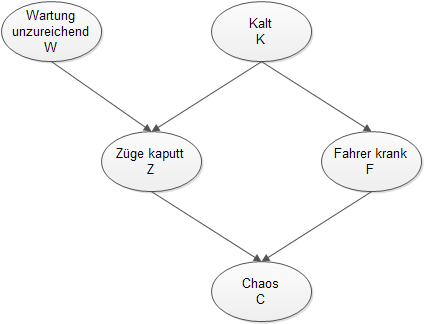
\includegraphics[width=0.5\columnwidth]{blatt5aufgabe4}
\end{figure}

\subsection*{4.b)}
Gesucht ist $\IP(C=w|K=w,Z=f)$. Es gilt
\begin{align}
	\IP(C=w|K=w,Z=f) &= 0.9 \cdot \IP(F=w|K=w) + 0.25 \cdot \IP(F=f|K=w) \notag \\
									 &= 0.9\cdot0.7 + 0.25\cdot0.1 \notag \\
									 &= 0.655 \notag \\
									 &= 65.5\% \notag 			 
\end{align}

\subsection*{4.c)}
Gesucht ist $\IP(K=w|F=w)$. Der Satz von Bayes gibt uns
\begin{align}
	                       & \IP(K=w|F=w) \cdot \IP(F=w) = \IP(F=w|K=w) \cdot \IP(K=w) \notag \\
	 \Leftrightarrow \quad & \IP(K=w|F=w) = \frac{\IP(F=w|K=w) \cdot \IP(K=w)}{\IP(F=w)} \notag
\end{align}

Einsetzen der totalen Wahrscheinlichkeit f\"ur $\IP(F=w)$ liefert dann
\begin{align}
	\IP(K=w|F=w) &= \frac{\IP(F=w|K=w) \cdot \IP(K=w)}{\IP(F=w)} \notag \\
							 &= \frac{\IP(F=w|K=w) \cdot \IP(K=w)}{\IP(F=w|K=w) \cdot \IP(K=w) + \IP(F=w|K=f) \cdot \IP(K=f)} \notag \\
							 &= \frac{0.7 \cdot 0.2}{0.7 \cdot 0.2 + 0.1 \cdot 0.8} \notag \\
							 &= 0.\overline{63} \notag \\
							 &= 63.\overline{63}\% \notag
\end{align}

\subsection*{4.d)}
Gesucht ist $\IP(W=w|Z=w)$. Der Satz von Bayes gibt uns
\begin{align}
	                       & \IP(W=w|Z=w) \cdot \IP(Z=w) = \IP(Z=w|W=w) \cdot \IP(W=w) \notag \\
	 \Leftrightarrow \quad & \IP(W=w|Z=w) = \frac{\IP(W=w|K=w) \cdot \IP(W=w)}{\IP(Z=w)} \notag
\end{align}

Einsetzen der totalen Wahrscheinlichkeit f\"ur $\IP(F=w)$ liefert dann
\begin{align}
	\IP(W=w|Z=w) &= \frac{\IP(Z=w|W=w) \cdot \IP(Z=w)}{\IP(Z=w)} \notag \\
							 &= \frac{\IP(Z=w|W=w) \cdot \IP(Z=w)}{\IP(Z=w|W=w) \cdot \IP(W=w) + \IP(Z=w|W=f) \cdot \IP(W=f)} \notag \\
							 &= \frac{\IP(Z=w|W=w) \cdot 0.7}{\IP(Z=w|W=w) \cdot 0.7 + \IP(Z=w|W=f) \cdot 0.3} \notag
\end{align}

Weiterhin gilt
\begin{align}
	\IP(Z=w|W=w) &= \IP(Z=w|W=w,K=w) \cdot \IP(K=w) + \IP(Z=w|W=w,K=f) \cdot \IP(K=f) \notag \\
							 &= 0.9 \cdot 0.2 + 0.6 \cdot 0.8 \notag \\
							 &= 0.66 \notag
\end{align}

sowie
\begin{align}
	\IP(Z=w|W=f) &= \IP(Z=w|W=f,K=w) \cdot \IP(K=w) + \IP(Z=w|W=f,K=f) \cdot \IP(K=f) \notag \\
							 &= 0.6 \cdot 0.2 + 0.1 \cdot 0.8 \notag \\
							 &= 0.2 \notag
\end{align}

Also insgesamt
\begin{align}
	\IP(W=w|Z=w) &= \frac{\IP(Z=w|W=w) \cdot 0.7}{\IP(Z=w|W=w) \cdot 0.7 + \IP(Z=w|W=f) \cdot 0.3} \notag \\
							 &= \frac{0.66 \cdot 0.7}{0.66 \cdot 0.7 + 0.2 \cdot 0.3} \notag \\
							 &\approx 0.885 \notag \\
							 &= 88.5\% \notag						 
\end{align}

\end{document}
